%%%%%%%%%%%%%%%%%%%%%%%%%%%%%%%%%%%%%%%%%
% LaTeX Template
% http://www.LaTeXTemplates.com
%
% Original author:
% Linux and Unix Users Group at Virginia Tech Wiki 
% (https://vtluug.org/wiki/Example_LaTeX_chem_lab_report)
%
% License:
% CC BY-NC-SA 3.0 (http://creativecommons.org/licenses/by-nc-sa/3.0/)
%
%%%%%%%%%%%%%%%%%%%%%%%%%%%%%%%%%%%%%%%%%

%----------------------------------------------------------------------------------------
%	PACKAGES AND DOCUMENT CONFIGURATIONS
%----------------------------------------------------------------------------------------

\documentclass[12pt]{article}
\usepackage{geometry} % Pour passer au format A4
\geometry{hmargin=1cm, vmargin=1cm} % 

\usepackage{graphicx} % Required for including pictures
\usepackage{float} % 

%Français
\usepackage[T1]{fontenc} 
\usepackage[english,francais]{babel}
\usepackage[utf8]{inputenc}
\usepackage{eurosym}
\usepackage{lmodern}
\usepackage{url}
\usepackage{multicol}

%Maths
\usepackage{amsmath,amsfonts,amssymb,amsthm}
%\usepackage[linesnumbered, ruled, vlined]{algorithm2e}
%\SetAlFnt{\small\sffamily}

%Autres
\linespread{1} % Line spacing
\setlength\parindent{0pt} % Removes all indentation from paragraphs

\renewcommand{\labelenumi}{\alph{enumi}.} % 
\pagestyle{empty}
%----------------------------------------------------------------------------------------
%	DOCUMENT INFORMATION
%----------------------------------------------------------------------------------------
\begin{document}

%\maketitle % Insert the title, author and date

\begin{minipage}[t]{\textwidth}
  \raggedright
      {\bfseries Série A}\\[.35ex]
      {\bfseries 1 STI 2D 2}\\[.35ex]
      {\bfseries Nom : }\\[.35ex]
      \vspace*{-1cm}
      \raggedleft
          {\bfseries Dérivées}\\[.35ex]
          {\bfseries 10 Mars 2015}\\[.35ex]
\end{minipage}\\[1em]

\begin{center}
  \textsf{Focus is a matter of deciding what things you're not going to do. - John Carmack}\\
\end{center}

\setlength{\columnseprule}{1pt}

\subsection*{I - Nombres dérivés}


\begin{figure}[H]
  \centering
  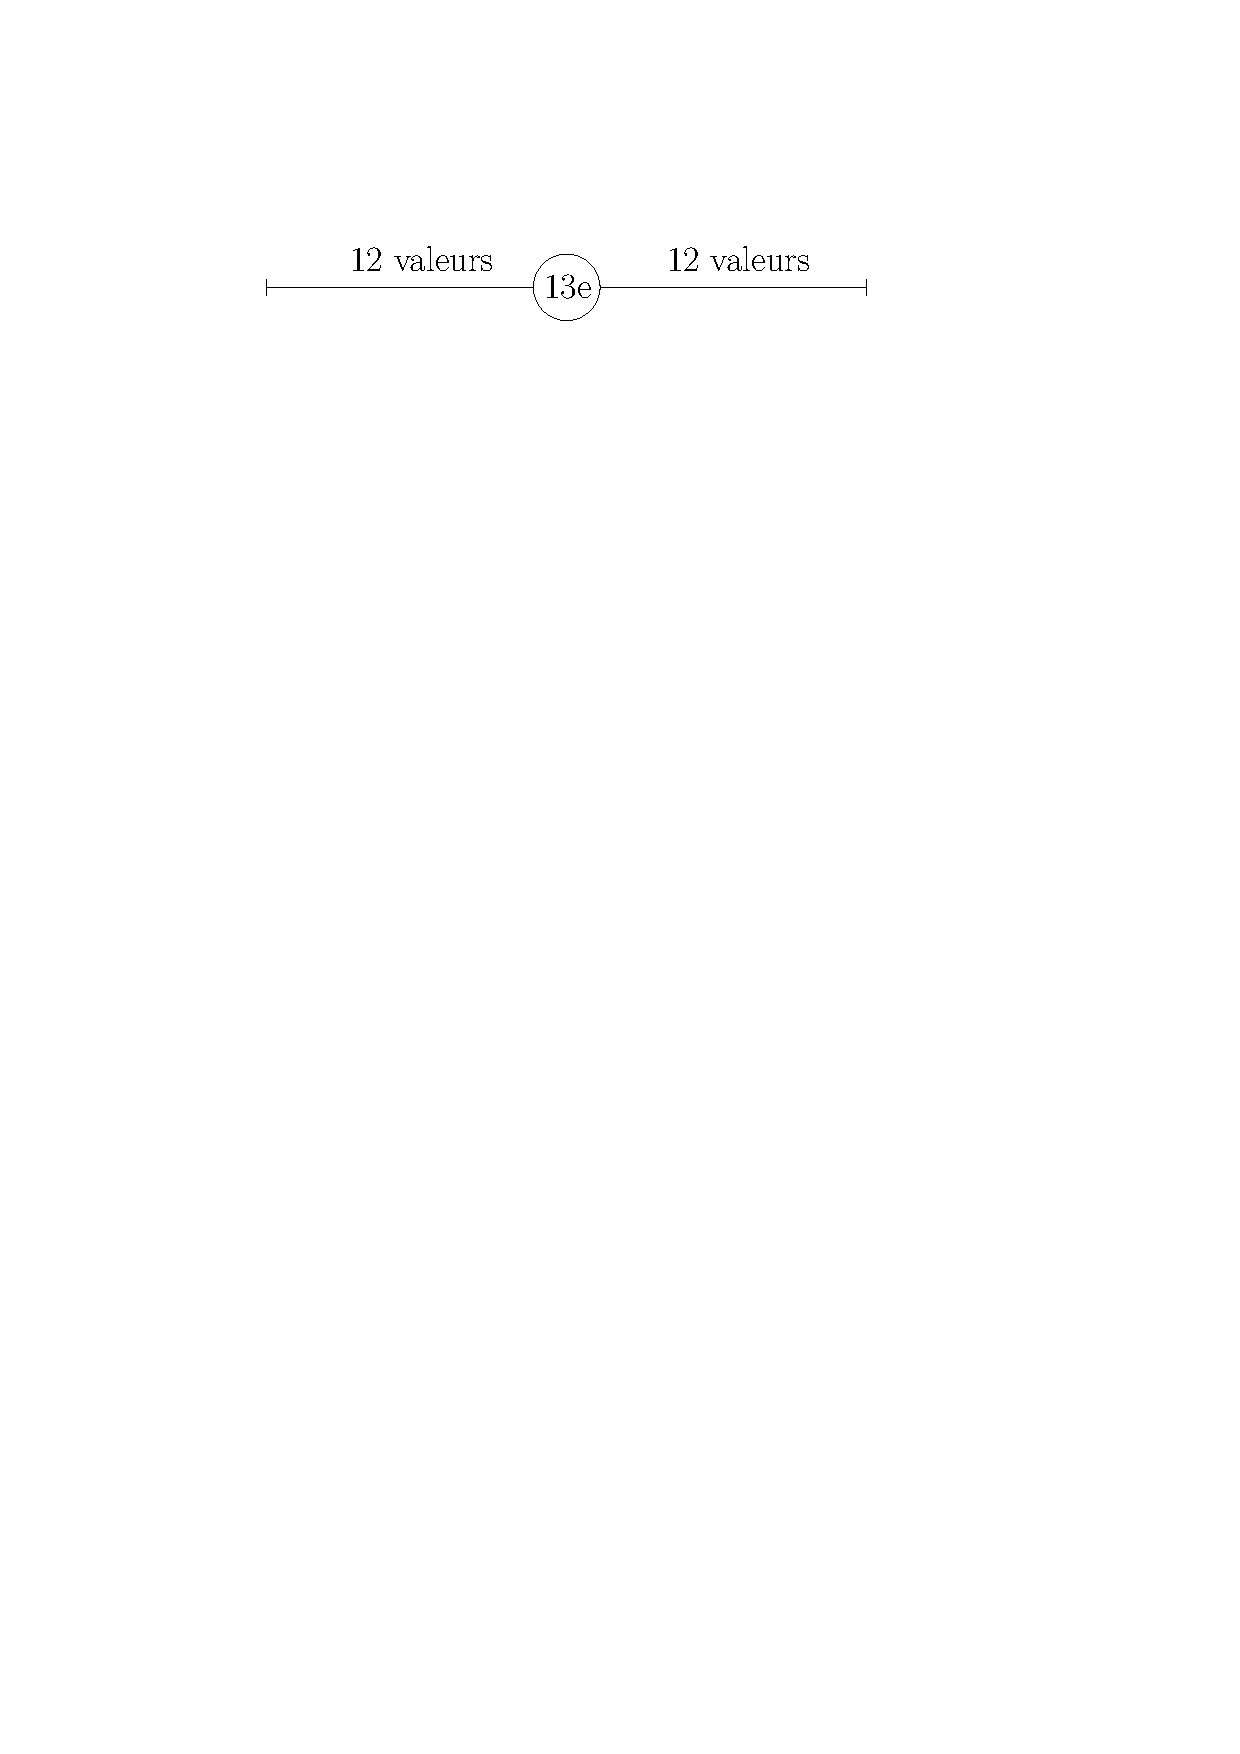
\includegraphics[width=\linewidth]{sources/ie/ex1.pdf}
\end{figure}

\begin{enumerate}
\item[1.] Donner $f(-2)$, $f(0)$ et $f(2)$.
\item[2.] Après avoir tracer les tangentes adéquates, donner $f'(-2)$, $f'(0)$ et $f'(2)$.
\item[3.] Compléter les phrases suivantes :
  \begin{itemize}
  \item Si la fonction dérivée $f'(x)$ est négative sur $[a, b]$ alors la fonction $f$ est ...
  \item Si la fonction dérivée $f'(x)$ est positive sur $[a, b]$ alors la fonction $f$ est ...
  \item Si la fonction dérivée $f'(x)$ est nulle sur $[a, b]$ alors la fonction $f$ est ...
  \end{itemize}
\end{enumerate}

\begin{multicols}{2}

\subsection*{II - Fonctions dérivées}
Calculer les fonctions dérivées des fonctions suivantes.
\begin{eqnarray*}
  f_{1}(x) &=& x - 3x^{2} + \sqrt{2}\\
  f_{2}(x) &=& \dfrac{7x^{3} - 2x}{2\pi}\\
  f_{3}(x) &=& (x^{2} - 1)x\\
  f_{4}(x) &=& \dfrac{3x - x^{3}}{3x+1}\\
  f_{5}(x) &=& \dfrac{x - 3}{x^{2} + 7}
\end{eqnarray*}

\subsection*{III - Étude de fonction}
Soit la fonction $f(x) = \dfrac{-2x-3}{x+3}$.

\begin{enumerate}
\item[1.] Calculer la fonction dérivée $f'(x)$.
\item[2.] À l'aide de l'étude du signe de la dérivée, étudier les variations de $f$.
\item[3.] Remplir le tableau de valeur ci-dessous :
\item[4.] Tracer la fonction $f$ dans le repère ci-dessous.
\end{enumerate}
\end{multicols}

  \begin{center}
    \begin{tabular}{| c | c | c | c | c | c | c | c |}
      \hline
      $x$ & -2 & -1 & 0 & 1 & 2 & 3 & 4\\
      \hline
      $f(x)$  & \phantom{123456789} & \phantom{123456789} & \phantom{123456789} & \phantom{123456789} & \phantom{123456789} & \phantom{123456789} & \phantom{123456789} \\
      \hline
    \end{tabular}
  \end{center}


  \begin{figure}[H]
    \centering
    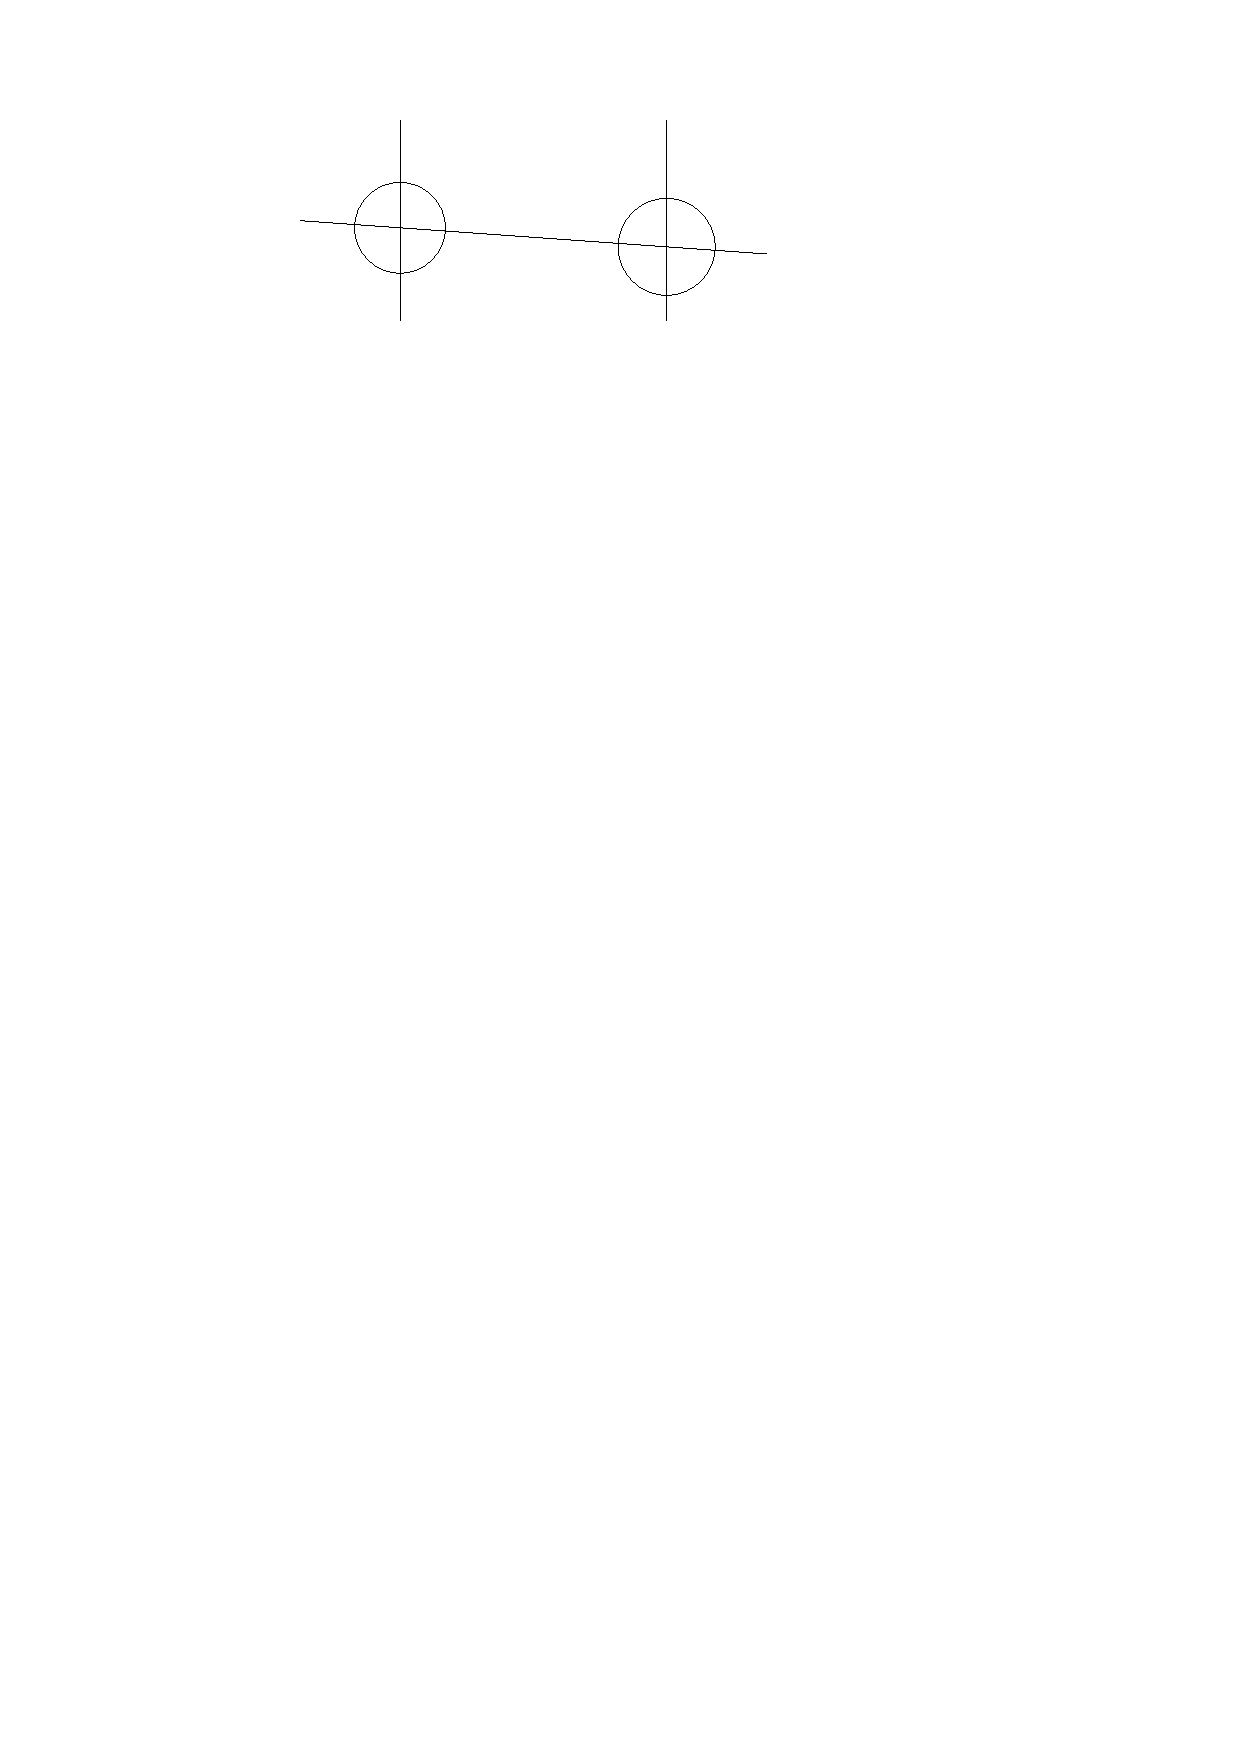
\includegraphics[width=\linewidth]{sources/ie/ex3.pdf}
  \end{figure}


\subsection*{IV - Bonus}

Calculer la fonction dérivée de $-\dfrac{-2\cos(-4x - 3)}{3}$.

\end{document}
